\documentclass{article}
\usepackage[utf8]{inputenc}
\usepackage{titling}
\usepackage{graphicx}
\usepackage{xcolor}
\usepackage[colorlinks=true,linkcolor=darkgray, urlcolor =gray]{hyperref}
\usepackage[spanish]{babel}
\DeclareUnicodeCharacter{301}{~}
\usepackage{url}
\usepackage{hyperref}


\title{Servicios Web}
\author{Cristina Díaz García}
\date{Enero 2019}

\renewcommand\maketitlehooka{\null\mbox{}\vfill}
\renewcommand\maketitlehookd{\vfill\null}


\begin{document}

\addcontentsline{toc}{section}{Índice general}

\begin{titlingpage}
\maketitle
\end{titlingpage}

\newpage

\tableofcontents

\newpage

\section{Introducción}


\section{Descripción de las tecnologías}

\subsection{Tecnologías para intercambio de datos}

\subsubsection{XML}

XML, eXtensible Markup Language, es parecido a HTML, y como éste, no es un lenguaje de programación, sino un lenguaje de marcado, usado para definir etiquetas con las que dar formato al texto o los datos que se quieran representar. Se suele usar en base de datos y software ofimático, aunque es posible usarlo para cualquier aplicación imaginable, ya que se creó sin ningún objetivo concreto más alla del intercambio de información estructurada entre plataformas.

Algunos de los usos más frecuentes son con las APIs, la migración de datos y las aplicaciones web. Un ejemplo de esto es \href{https://cloud.google.com/storage/docs/xml-api/overview}{la API de Google Cloud}.

\begin{center}
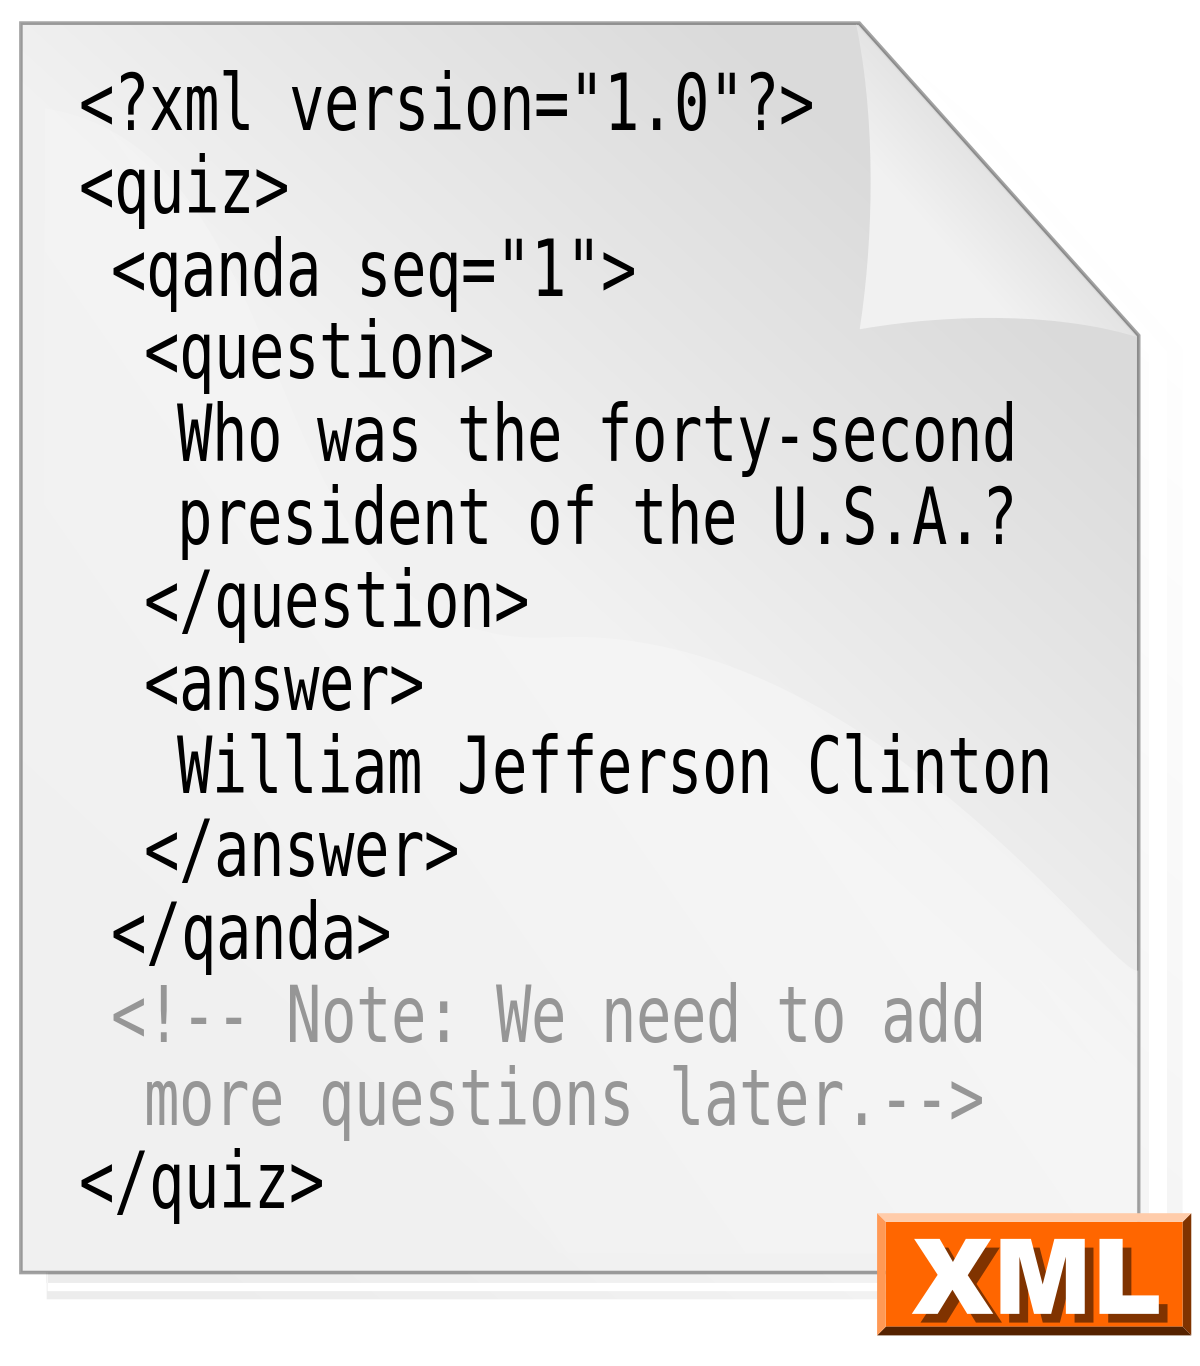
\includegraphics[scale=0.07]{images/XML.png}
\end{center}

\subsubsection{JSON}

JSON, JavaScript Object Notation, es un lenguaje de marcado, al igual que XML, aunque se diferencia de este en su formato, que es más ligero, más sencillo: no tiene etiquetas complejas sino que se compone de pares clave-valor. También es más fácil de analizar usando funciones de JavaScript, que se usa en casi cualquier navegador web. Es esto lo que hace que sea muy buena alternativa a XML.

Los usos de JSON son muy similares a los de XML, como las APIs, de distintos lenguajes como \href{https://docs.python.org/2/library/json.html}{Python} o \href{https://common-lisp.net/project/cl-json/cl-json.html}{Lisp}. También Google Cloud tiene una \href{https://cloud.google.com/bigquery/docs/loading-data-cloud-storage-json}{acepta JSON}.

\begin{center}
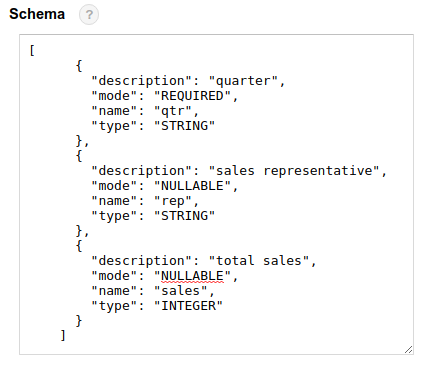
\includegraphics[scale=0.3]{images/json.png}
\end{center}

\subsection{Protocolos para intercambio de datos estructurados}

\subsubsection{SOAP}

SOAP, Simple Object Access Protocol, es un protocolo por el cual se intercambian archivos XML. Se usa mayormente en servicios web, y solo soporta XML, en ningún caso JSON. Un ejemplo de uso de SOAP es \href{http://www.juntadeandalucia.es/servicios/madeja/contenido/recurso/41}{el Marco de Desarrollo de la Junta de Andalucía}.

\begin{center}
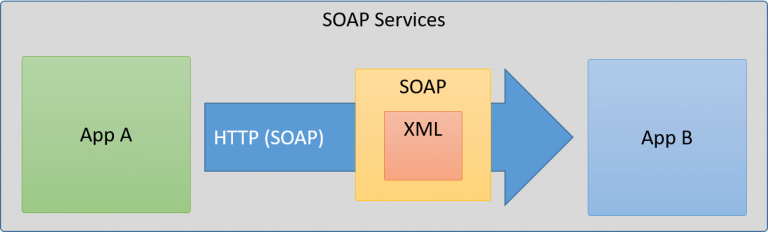
\includegraphics[scale=0.4]{images/soap.png}
\end{center}

\subsection{Estilos arquitectónicos}

\subsubsection{SOA}

SOA, Service-Oriented Architecture, es un tipo de arquitectura que apoya la integración de aplicaciones a través de \textit{servicios}, que son actividades que cubren necesidades dell usuario. Es, por así decirlo, la entidad que encapsula tanto SOAP como REST.

\begin{center}
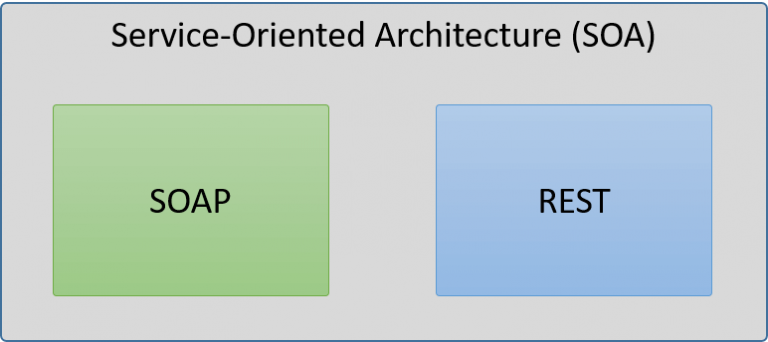
\includegraphics[scale=0.3]{images/soa.png}
\end{center}

En nuestra vida diaria usamos SOA, por ejemplo, cuando hacemos alguna transacción con la tarjeta de crédito/débito y en general, en cualquier transacción económica cuya facturación es a tiempo real.

\subsubsection{REST}

REST, REpresentational State Transfer, es un estilo de aquitectura software usada para transportar casi cualquier tipo de datos. Al contrario que SOAP, que solo podía transmitir archivos XML, REST funciona con XML, JSON, texto, imágenes...

\begin{center}
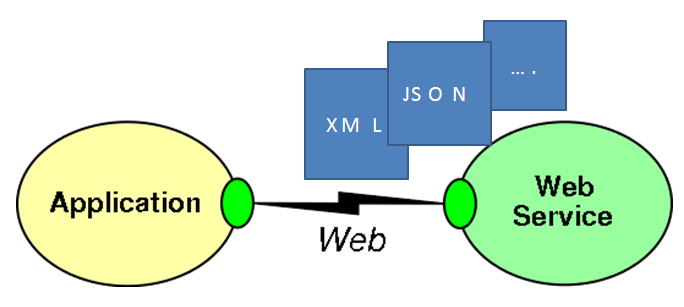
\includegraphics[scale=0.3]{images/rest.png}
\end{center}

Un ejemplo de uso de REST a día de hoy son las Aplicaciones de Google (Firebase, Drive...)

\section{Conclusión personal}
En mi opinión, todas estas tenologías son, sin duda, útiles. En la primera sección, aunque es cierto que XML es muy útil para definir estructuras complejas en comparación con JSON, y es mucho más reestructurable, JSON da una flexibilidad que considero superior a la hora de comparar qué tecnología usar, y como se suele decir, \textit{simpler is better}. Es por ello que si tuviera que decidir, en general, usaría JSON.
Por ese motivo, también si tuviera que decidir entre REST y SOAP, elegiría REST, ya que SOAP te limita a XML, y REST no solo te permite usar XML sino muchos otros formatos y archivos.
Finalmente, el uso de servicios con SOA también me parece bastante adecuado, ya que permite usar tanto REST como SOAP, para las personas que quieran usar cualquiera de los dos.

\begin{thebibliography}{9}
\bibitem{ExtensibleMarkupLanguage} Extensible Markup Language, \url{https://es.wikipedia.org/wiki/Extensible_Markup_Language}.
\bibitem{UsosXML} Usos de XML, \url{https://desarrolloweb.com/articulos/460.php}.
\bibitem{APIXML} How to connect to an API and parse XML (and why you would want to), \url{http://www.netinstructions.com/how-to-connect-to-an-api-and-parse-xml-and-why-you/}.
\bibitem{JSON} JSON, \url{https://es.wikipedia.org/wiki/JSON}.
\bibitem{SOAP} SOAP, \url{https://es.wikipedia.org/wiki/Simple_Object_Access_Protocol}.
\bibitem{SOAPvsREST} SOAP vs REST, \url{https://www.oscarblancarteblog.com/2017/03/06/soap-vs-rest-2/}.
\bibitem{SOA} SOA, \url{https://es.wikipedia.org/wiki/Arquitectura_orientada_a_servicios}.
\bibitem{UsosSOA} SOA en nuestra vida diaria, \url{https://www.megapractical.com/blog-de-arquitectura-soa-y-desarrollo-de-software/soa-en-nuestra-vida-diaria}.
\bibitem{REST} REST, \url{https://es.wikipedia.org/wiki/Transferencia_de_Estado_Representacional}.
\end{thebibliography}



\end{document}